%!TEX TS-program = lualatex

\documentclass[twocolumn,2pt]{article}

\usepackage{geometry}
\usepackage{graphicx, subcaption, setspace, booktabs, float}

\geometry{left=2.3cm, right=2.3cm}

\title{Data Challenge: Geolocation of Connected Devices}

\author{Valentin Charvet, Maxence Monfort}




\begin{document}
	\maketitle
	\hspace{2cm}
	
	
	\textit{This document presents the results of a data-challenge as part of IA317 Large Scale Machine Learning course from Artificial Intelligence Master (Télécom ParisTech and ENSTA ParisTech). The study consists in geolocating connected devices based on the send signals.}	
	\footnote{Full code available at https://github.com/vcharvet/geoloc-challenge }
		
		%Ce document présente les résultats du challenge du cours IA317 Large Scale Machine Learning du master Intelligence Artificielle (Télécom ParisTech et ENSTA ParisTech). L'étude consistait à géolocaliser des objets connectés à partir des paramètres des signaux qu'ils ont envoyés et de la manière dont ils ont été réceptés par un réseau d'antennes. Nous avons séparé ce travail en deux parties, dans un premier temps nous avons estimé les distances séparant les objets des antennes, puis nous avons à partir de ces informations prédit la localisation de chacun des objets.
	
	\section{Introduction}
	Along with the rise of the number of connected devices during the last decade (mobile phones, IOT etc...), questions have been raised with report to the geolocalization of those, that is finding accurate coordinates. Such information can be very useful for many applications and thus lead to many interests in industries and services. As a consequence, the research community has produced a number of publications as shown in survey \cite{roxin:hal-00470120}.
	
	The problem at stake is the following: given a network of $M$ base stations (or antennas) and a set of $N$ messages received by the stations, how can one retrieve the latitude and longitude of each emitting device? Let's precise that each message can be received by several antennas and can be in motion meaning we want to predict the device's coordinates at the time of message emission.
	
	However, many publications related to this problem restrict their study to the localization of objects in a closed environment like a house for which the receiving devices are relatively close to the emitter (less than 100 meters) as in \cite{he2013testbed}. Unfortunately, those don't apply to our dataset since our distance is centered around $6.6$ km with a standard deviation of $13.4$, see  Fig \ref{distance_distrib}.
	
	Moreover, the high number of samples as well as the uncertainty of the measurements has led us to think a statistical method would be appropriate. Consequently, we based our predictions on a machine learning two-target regression model. In section \ref{methods} we describe the process of feature engineering necessary to obtain an interpretable feature matrix. We also describe methods and approximations we have made to estimate distances between devices and antennas. In section \ref{results} we show the empirical results of our studies and then in \ref{conclusion} we conclude.

	\begin{figure}[H]
		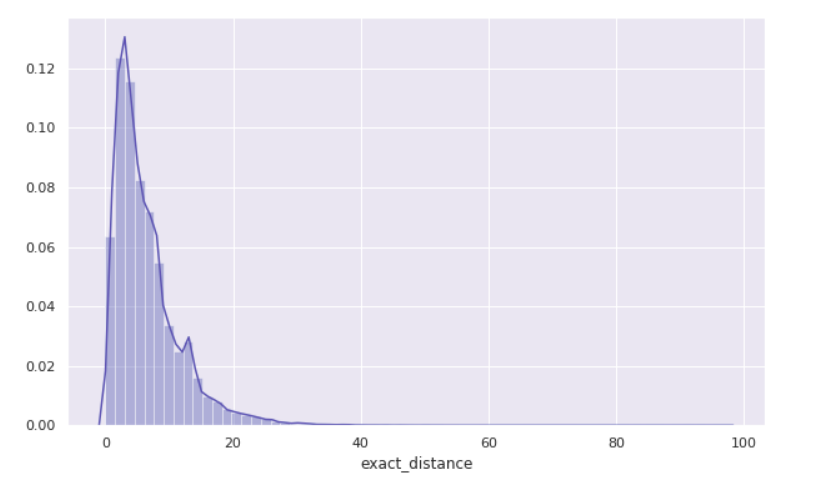
\includegraphics[width=9cm, height=6cm]{graphes/distance_distrib.png}
		\caption{Distribution of distances smaller than 100km}
		\label{distance_distrib}		
	\end{figure}
	\vspace{-20pt}


	\section{Methods and Data Description}
	\label{methods}
	\subsection{Data}
	Our training data consists in a set of $11 072 334$ messages received by a network of $159$ base stations. Each entry describes the unique id of the message (received by several antennas) and various parameters, along which $rssi$ (Received Signal Strength Indicator), and $frequency$. In addition, we have at our disposition the coordinates of the base stations.
	
	Each received message comes with a variety of features, some are proper to the emitting device for instance $motion$: we call them $client_features$. The others are proper to the antenna like $time_{ux}$: we call those $bs_{features}$. Consequently, to retrieve a feature vector for each message, we have to concatenate the $client_features$ with all the $bs_features$ relative to this message. Let's denote $p_1$ and $p_2$ the number of client and bs features respectively, the shape of the final feature vectors will be 
	\begin{equation}
		\label{feature_number}
		P= p_1 + 159 \times p_2
	\end{equation}
	 as there are $159$ base stations. We proceed to this task using the class \textbf{Builder} from \textbf{utils.feature\_builder.py}. As the computation cost for this is quite expensive, we perform it in a serialized way to reduce the execution time. Parsing the whole database with this class is usually done in less than a hour.
	
	
	\subsection{Methods}
	\label{methods}
	Even though we have a lot of features for each message, $P>100$ when using all features with parsing technique explained in previous section, they are not really consistent for the regression task on predicting latitude and longitude: a first submission return a criterion greater than 14km ! In order to overcome this issue, we decided to estimate the distances from device to antennas, and input them into each feature vector. We tried 4 different methods for this purpose. Three of them are based on parametric estimation of the $rssi$ using ordinary least squares, and the other based on a fully connected neural network.
	
	
	\subsubsection*{Basic rssi}
	Starting with a simple model taken from \cite{srbinovska2011localization} section IV, we write rssi as 
	\begin{equation}
	\label{naive_rssi}
		rssi = A - 10 n log(d) 
	\end{equation}
	where $rssi$ is the received signal strength at base station (dB), $A$ and $n$ are the estimated parameters and $d$ is the distance (meters) between the device and the base station. $d$ is calculated with geopy python package using coordinates of devices and base stations.
	
	That means for each base station, we minimize the following objective function:
	\begin{equation}
	\label{naive_rssi_objective}
	f_i(n, A) = \frac{1}{n_i} \sum_{j=1}^{n_i} (rssi_{ij} -A + 10 \ n \ log(d_{ij}))^2
	\end{equation}
	where $i=1\dots 159$ indicated the base station, $n_i$ the number of messages received by the bs, $d_ij$ the distance between base station $i$ and message $j$
	
	
	\subsubsection*{Augmented rssi}
	To improve the previous model we use equation (3) from \cite{Chiputa2018}
	\begin{equation}
	\label{augmented_rssi}
	rssi = rssi_0 - 10 n log(\frac{d}{d_0}) + err
	\end{equation}
	For the estimation, we will regroup $rssi_0$ and $err$ in a unique term $A$ and using the same notation as before, we write the objective function as:
	\begin{equation}
	\label{augmented_rssi_objective}
	f_i(n, d_0, A) = \frac{1}{n_i} \sum_{j=1}^{n_i} (rssi_{ij} -A + 10 \ n \ log(\frac{d_{ij}}{d_0}))^2
	\end{equation}
	
	
	\subsubsection*{Frequency-based rssi} 
	\begin{equation}
	\label{freq_rssi}
	rssi = rssi_0 + 10 \ n \ log(d \times f) - 30n + C
	\end{equation}
	
	$C$ is a propagation constant we also try to estimate even though a common used value is 32.44, $f$ is the frequency of the received signal (MHz) %TODO find reference
	This yield the following objective:
	
	\begin{equation}
	\label{freq_rssi_objective}
	f_i(n, rssi_0, C) = \frac{1}{n_i} \sum_{j=1}^{n_i} (rssi_{ij} - rssi_0 + 10n \ log(d \times f) - 30n + C)^2
	\end{equation}
	
	%TODO ref to scipy
	We have used the module \textbf{scipy.optimize.minimize} for the estimation of parameters of the objective function described above. To overcome convergence to wrong solutions, we have constrained the value of $rssi_0$ to be greater than $max(rssi_{ij})_{j=1 \dots n_i}$ for physical consistence (the value of the sent signal can't be less than the received one). The scripts for these estimation are available at \textbf{mains/rssi\_params.py} .
	
	Once the estimation of the parameters is done, we can estimate the distance of a new device using equations (\ref{naive_rssi}), (\ref{augmented_rssi}) and (\ref{freq_rssi}).
	
	
	\subsubsection*{Neural-based Estimation} %TODO ref representation theorem
	As we have struggled finding good estimations of distances with parametric models, we tried estimated the distance with a multi-layer perceptron regressor \cite{Cybenko1989}. Theoretically, such an estimator can approximate any real-valued function. Finding inspiration with parametric models described above, we tried to estimate the function $f$ such that
	$$ f(lat_{bs}, lng_{bs}, freq, rssi) = d $$
	
	That model consists in training a MLP regressor with the target $d$ and predictors $lat_{bs}, \ lng_{bs}, \ freq \ $and$ \ rssi$ 
	%TODO cite keras
	We have done this part with keras and tried different layer configurations and regularization parameters.
	
	
	\subsubsection*{Infering devices coordinates}
	%TODO references for feature selection
	This part is the least complicated provided we have found the most adequate features in the previous tasks. However, as we find ourselves with a great number of features (\ref{feature_number}), we need to select the bet among them. As we are working in a two-target regression framework, many of the statistical tests are not applicable. Even though there exist ways to work around this, we chose simpler methods. 
	
	As our feature matrix is sparse, we put a mask over the columns to select only the ones with a number of non-zero values greater than a treshold. The latter has been tuned by cross-validation.
	
	We also assumed the regression model would struggle training on outlier values ie targets for which the latitude or longitude is "far" from the mean: we removed the training values where $ x \notin \lbrack \bar{x} \pm k \times \sigma_x \rbrack $ where $x$ is longitude or latitude, $\bar{x}$ the mean, $\sigma_x$ the standard deviation and k is a tuned hyper-parameter.
	
	The best regressors we found were random forests and xgboost. The final predictions were made with those, with parameters tuned by bayesian optimization with hyperopt python package \cite{hyperopt}.
	
	
	\section{Results}
	\label{results}
	
	\subsection*{Distance Estimation}
	Among all the techniques we used for estimating the distance using available parameters, the best was the one using MLP regression. We assume this is due to the fact that the formulas given in section \ref{methods} for rssi were not consistent for the wide range of distance in our dataset. They would have probably worked well for small distances only. Hence, that is the MLP estimation of the distance we used for the final predictions.
	
	\subsection{Coordinates prediction}
	
	
	We present our results in the table \ref{results_tab}.
	\begin{itemize}
		\item \textit{algorithms}, Random Forest (RF) or XGBoost
		\item \textit{$n_{features}$}, number of features, we keep features that have a number of non-zeros greater than a treshold
		\item \textit{mask}, range of the targets
		\item \textit{CV loss}, cross validated score on 5 folds.
	\end{itemize}
	
	\begin{tabular}{c | c | c | c}
		\label{results_tab}
		Algorithm & $n_{feature}$ &mask & CV loss (k=5) \\
		\hline
		RF & 659 & None & 4.9 \\
		RF &659 & $\bar{x} \pm \sigma$ & 4.8 \\
		RF & 209 & $\bar{x} \pm  \sigma$ &  6.7 \\
		RF & 450 & $\bar{x} \pm  \sigma$ & 4.8 \\
		XGBoost & 659 & $\bar{x} \pm  \sigma$ & \textbf{4.6} \\
		XGBoost & 450 & $\bar{x} \pm  \sigma$ & \textbf{5.6} \\
		\hline		
	\end{tabular}
	\newline

	Out best regressor was xgboost with $max_{depth} = 30$ and $100$ estimators. It gave a test score of $6.63 \ km$.
	
	\section{Conclusion}
	\label{conclusion}
	Thanks to our efficient feature engineering and selection methods, we achieved a final prediction among the best of the challenge. However, the criterion is still quite large ($6.63 \ km$). 
	
	With more time, we could have managed to improve the prediction. In particular, we think we could have obtained better estimation of the device-antenna distances with better tuning of our neural network or $rssi$ formulas better suited to the range of distances.
	
	
	
	\bibliography{rapport}
	\bibliographystyle{plain}
\end{document}